\chapter{Project and project management}\label{chap:intro}
\fancyhead[R]{Project and project management}

\textit{``This chapter provides a comprehensive overview of the project context, including the host organization presentation, problem statement, project objectives, and the management methodology employed. It establishes the foundation for understanding the real-time fee calculation system development within the P2S financial platform.''}

\pagebreak

\section{Introduction}

The French electronic payment ecosystem presents significant challenges for financial institutions in processing transaction fees from international payment networks. These challenges stem from both structural complexities in fee determination and computational inefficiencies in current processing systems. This project addresses these challenges through the development of an integrated framework that combines systematic fee structure normalization with high-performance computational engines.

The project is part of the Payment Steering Solution (P2S) initiative, which aims to enhance fee calculation accuracy and efficiency through a robust two-tier architecture. This architecture consists of a Document Normalization Layer that standardizes heterogeneous fee rules, and a Transaction Processing Layer that applies these rules efficiently in real-time environments.

The primary focus of this thesis is the design and implementation of stateless computational engines capable of processing high-volume transaction streams while maintaining accuracy and compliance with payment scheme regulations. These engines operate on pre-normalized fee structures to achieve optimal performance characteristics that would be impossible with traditional real-time document parsing approaches.

\section{Project Context and Motivation}

The French electronic payment ecosystem operates within a complex regulatory framework involving multiple stakeholders including issuing banks, acquiring banks, payment schemes, and regulatory authorities. Financial institutions must navigate intricate fee schedules, interchange rates, and processing charges that vary significantly based on transaction type, merchant category, geographic location, and numerous other parameters.

\subsection{Current Challenges in Fee Processing}

The calculation and validation of transaction fees present significant operational challenges that manifest in two primary domains:

\textbf{Structural Complexity:} Payment schemes distribute fee specifications through inconsistent documentation formats, predominantly as unstructured PDF documents exceeding several hundred pages. These documents contain embedded tabular data, conditional logic expressed in natural language, and complex cross-references that resist systematic computational interpretation without prior normalization.

\textbf{Computational Limitations:} Traditional fee calculation systems rely on monolithic architectures with hard-coded logic, resulting in several critical limitations:

\begin{itemize}
   \item \textbf{Performance Degradation:} Processing throughput exhibits inverse correlation with rule complexity, creating bottlenecks in high-volume environments
   \item \textbf{Maintenance Overhead:} Manual interpretation and hard-coding of fee rules creates maintenance complexity that scales poorly with specification update frequency
   \item \textbf{Scalability Constraints:} Monolithic frameworks lack the modularity necessary for dynamic scaling and efficient resource utilization
   \item \textbf{Processing Inflexibility:} Existing systems cannot efficiently leverage normalized data structures when available
\end{itemize}

\subsection{Business Impact}

These limitations result in measurable business impacts for financial institutions:

\begin{itemize}
   \item Increased operational costs due to manual fee validation processes
   \item Reduced transaction processing capacity during peak periods
   \item Higher risk of fee calculation errors and compliance issues
   \item Limited ability to adapt quickly to new payment scheme requirements
   \item Suboptimal resource utilization requiring over-provisioning of computational infrastructure
\end{itemize}

\subsection{Solution Approach}

This project addresses these challenges through an integrated framework comprising two complementary components:

\textbf{Normalization Framework:} Transforms heterogeneous payment scheme documentation into standardized, computationally-optimized data structures while preserving the semantic integrity of fee determination logic.

\textbf{Stateless Computational Architecture:} Leverages normalized data structures through dedicated, high-performance processing engines designed for optimal fee determination in real-time environments.

The architectural integration between these components enables horizontal scalability, fault isolation, and optimized resource utilization while eliminating real-time parsing overhead during transaction processing.

\section{Presentation of the Host Organization}

Effyis Group is a management and technology consulting firm founded in 2015 and headquartered in Paris, France. The company operates as a SARL (Limited Liability Company) with a capital of 150,000€ and reported revenue of 8.8M€ in 2020. With approximately 150 employees across two continents, Effyis positions itself as a medium-sized enterprise specializing in digital transformation for financial services.

\subsection{Organizational Structure}

Effyis Group operates with a flat organizational structure that minimizes management layers between executives and staff. This approach enables faster decision-making, more direct communication, and greater employee autonomy. Teams are formed dynamically based on project requirements, duration, and complexity rather than rigid hierarchical structures.

\subsection{Business Divisions}

The company operates through four main business divisions:

\begin{itemize}
    \item \textbf{Consulting:} Strategic planning, implementation assistance, and change management services for organizational transformation projects
    \item \textbf{Digital Factory:} Web and mobile application development using agile methodologies and customer-centered design approaches
    \item \textbf{Data Lab:} Data analytics services including strategy development, data science, governance frameworks, and visualization solutions
    \item \textbf{Payment:} Payment systems implementation, integration, platform certification, and regulatory compliance services
\end{itemize}

\subsection{Industry Specialization}

Effyis Group focuses on several key sectors:

\begin{itemize}
    \item \textbf{Banking:} Comprehensive services covering retail, corporate, private, and investment banking operations
    \item \textbf{Payment:} Support for banks, payment institutions, fintech companies, and startups in developing innovative payment solutions
    \item \textbf{Industry:} Operational optimization for pharmaceutical, automotive, telecommunications, and transportation companies
    \item \textbf{Insurance:} Digital transformation support through strategic planning, organizational restructuring, and innovation projects
\end{itemize}

\subsection{Key Products}

Effyis Group has developed several proprietary solutions:

\begin{itemize}
    \item \textbf{Lodin:} An open banking platform providing AISP and PISP functionalities for secure financial data exchange and payment processing
    \item \textbf{Payment Steering Solution (P2S):} A payment processing optimization system that analyzes and predicts interchange and scheme fees for financial institutions, including comprehensive billing management capabilities
\end{itemize}

\subsection{Company Profile}

\begin{table}[ht]
    \centering
    \begin{tabular}{|l|l|}
        \hline
        \textbf{Attribute} & \textbf{Details} \\
        \hline
        Company Name & EFFYIS Group \\
        \hline
        Founded & 2015 \\
        \hline
        Legal Structure & SARL (Société à Responsabilité Limitée) \\
        \hline
        Business Focus & Management and Technology Consulting \\
        \hline
        Company Size & 150 employees across 2 continents \\
        \hline
        Headquarters & 140 bis rue de Rennes 75006, PARIS \\
        \hline
        Capital & 150,000€ \\
        \hline
        Annual Revenue & 8.8M€ (2020) \\
        \hline
    \end{tabular}
    \caption{EFFYIS Group Company Information}
\end{table}

\section{Payment Industry Overview}

The payment industry encompasses a complex ecosystem of infrastructure, institutions, and processes that facilitate monetary value transfer between transacting parties. Understanding this ecosystem is essential for appreciating the technical challenges addressed by this project.

\subsection{Transaction Lifecycle}

Payment transactions follow a three-phase lifecycle:

\begin{figure}[H]
    \centering
    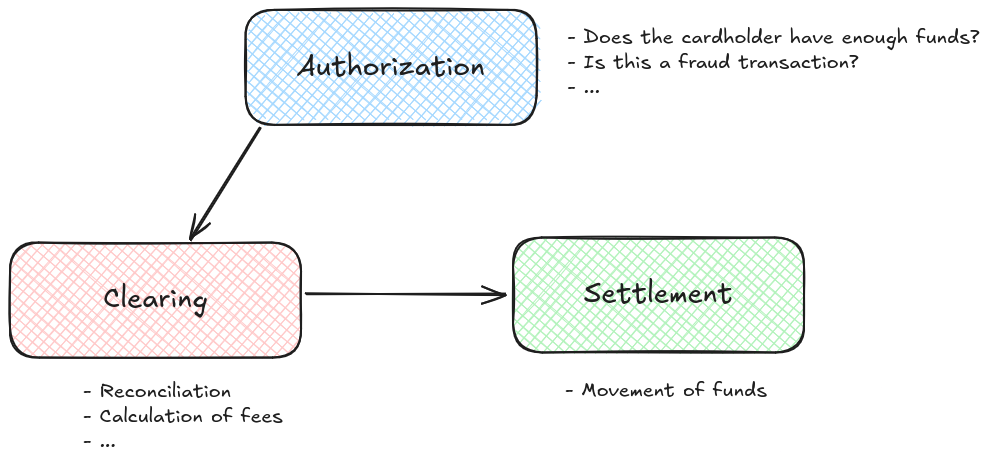
\includegraphics[width=0.8\textwidth]{img/Txn_Phases.png}
    \caption{Payment Transaction Lifecycle}
\end{figure}

\begin{itemize}
   \item \textbf{Authorization:} Real-time verification of payment credentials against predetermined criteria, including account status, available funds, and fraud indicators. This process typically executes within milliseconds, culminating in approval or rejection.
   
   \item \textbf{Clearing:} Administrative process for exchanging transaction data between participating financial institutions, including reconciliation procedures, fee calculations, and settlement instruction preparation. Clearing typically operates on batch processing schedules.
   
   \item \textbf{Settlement:} Final transfer of monetary value between financial institutions through established financial networks, often facilitated by central monetary authorities or specialized settlement entities.
\end{itemize}

\subsection{Ecosystem Participants}

The payment ecosystem comprises several key participants:

\begin{itemize}
   \item \textbf{Consumer:} Transaction initiator using payment credentials linked to accounts at issuing institutions
   \item \textbf{Merchant:} Commercial entity accepting payment for goods or services
   \item \textbf{Issuer:} Financial institution responsible for credential issuance and consumer account maintenance
   \item \textbf{Acquirer:} Financial institution providing payment acceptance services to merchants
   \item \textbf{Card Network:} Infrastructure provider establishing connectivity between issuers and acquirers
\end{itemize}

\begin{figure}[H]
    \centering
    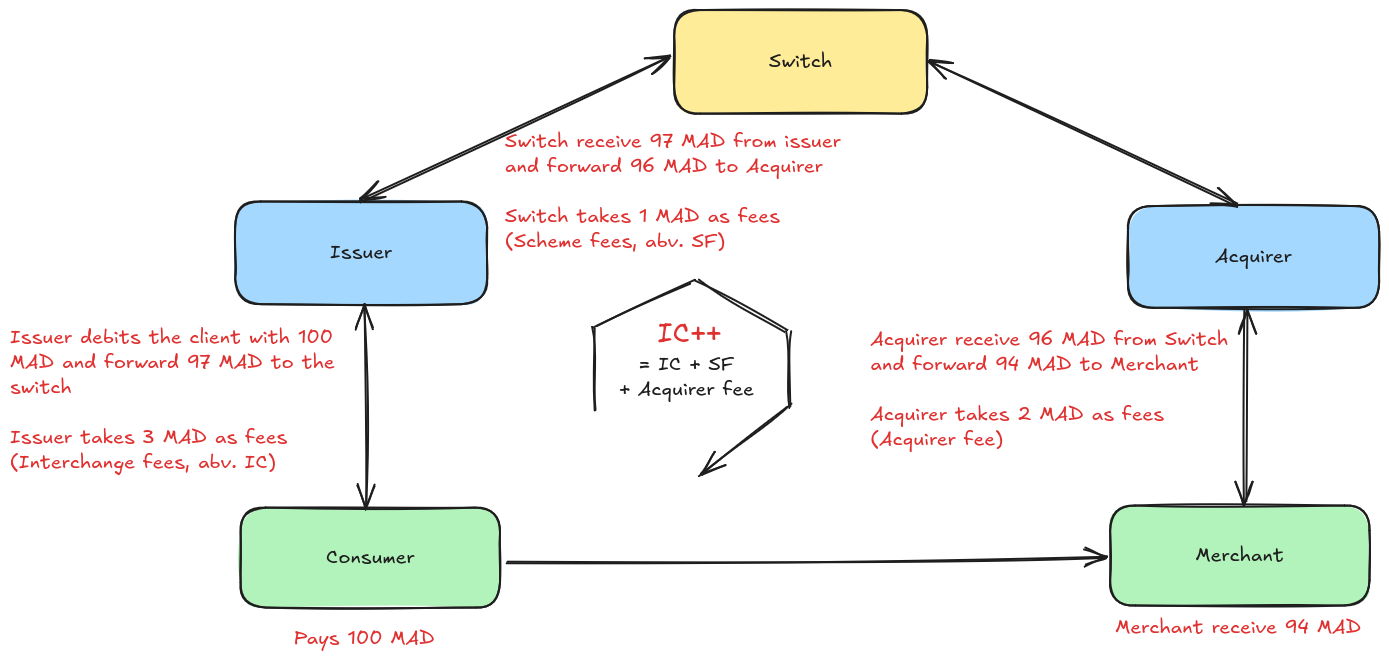
\includegraphics[width=\textwidth]{img/Txn_Actors.png}
    \caption{Payment Ecosystem Participants and Fee Flow}
\end{figure}

\subsection{Fee Structure}

The payment ecosystem operates on a multi-party fee structure:

\begin{itemize}
   \item \textbf{Interchange Fee:} Compensation from acquirers to issuers for each transaction, incentivizing credential issuance and compensating for credit risk
   \item \textbf{Scheme Fee:} Compensation to card networks for infrastructure services, financing network operations and fraud detection systems
   \item \textbf{Acquirer Fee:} Compensation retained by acquirers for merchant services, covering processing costs and risk management
\end{itemize}

\subsection{Messaging Architectures}

Two principal messaging architectures are employed:

\begin{figure}[H]
    \centering
    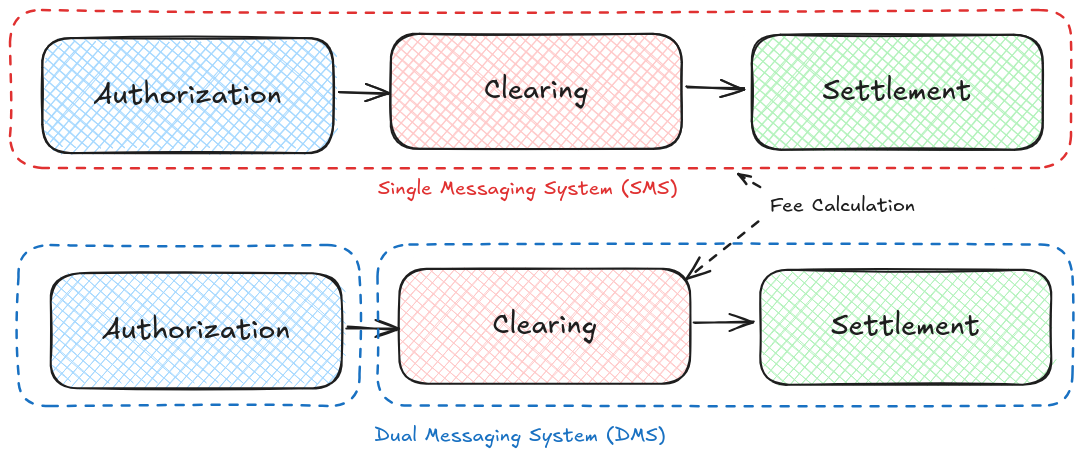
\includegraphics[width=0.8\textwidth]{img/Txn_SMS_DMS.png}
    \caption{Single and Dual Messaging Systems}
\end{figure}

\begin{itemize}
   \item \textbf{Single Messaging System (SMS):} Unified communication pathway processing authorization, clearing, and settlement concurrently in real-time
   \item \textbf{Dual Messaging System (DMS):} Separate authorization and clearing phases, enabling complex transaction scenarios and delayed settlement
\end{itemize}

\section{Problem Statement}

This project addresses a fundamental inefficiency in contemporary payment processing systems that manifests through two interconnected challenges affecting the French financial infrastructure.

\subsection{Primary Problem}

Financial institutions face significant operational inefficiencies when processing transaction fees from international payment networks due to:

\textbf{Structural Heterogeneity:} Payment schemes distribute fee specifications through inconsistent documentation formats that resist systematic computational interpretation. These documents, typically exceeding several hundred pages, contain embedded tabular data, conditional natural language expressions, and complex cross-references that require manual interpretation and hard-coding of fee logic.

\textbf{Computational Bottlenecks:} Traditional processing architectures demonstrate exponential performance degradation as rule complexity increases. Current systems exhibit:
\begin{itemize}
   \item Processing latency that scales poorly with rule complexity
   \item Resource contention in shared processing environments
   \item Sequential rule evaluation that cannot leverage parallel processing
   \item Inability to efficiently utilize normalized data structures
\end{itemize}

\subsection{Business Impact}

These limitations result in measurable operational impacts:

\begin{itemize}
   \item \textbf{Increased Processing Costs:} Manual validation processes and over-provisioned infrastructure
   \item \textbf{Reduced Throughput:} Performance bottlenecks during peak transaction periods
   \item \textbf{Compliance Risk:} Higher probability of fee calculation errors and regulatory violations
   \item \textbf{Operational Inflexibility:} Limited ability to adapt to changing payment scheme requirements
\end{itemize}

\subsection{Technical Challenges}

The compound nature of these challenges requires a comprehensive solution addressing both structural and computational dimensions:

\begin{itemize}
   \item Transformation of heterogeneous documentation into standardized, machine-readable formats
   \item Development of high-performance computational engines optimized for normalized rule application
   \item Implementation of scalable architecture supporting real-time processing requirements
   \item Integration with existing payment processing infrastructure
\end{itemize}

\section{Project Scope}

This project encompasses the design, implementation, and validation of an integrated framework for real-time fee calculation within the French payment ecosystem, focusing specifically on Visa and Mastercard fee structure optimization within the existing P2S platform infrastructure.

\subsection{Project Framework}

The complete framework consists of two interconnected components:

\subsubsection{Rule Normalization Framework}
Systematic transformation of heterogeneous payment scheme documentation into standardized, computationally-optimized data formats while preserving semantic integrity of fee determination logic.

\subsubsection{Stateless Computational Engine Architecture}
High-performance processing engines operating on normalized data structures to achieve optimal fee determination in real-time environments. This component represents the primary focus of this thesis.

\subsection{Thesis Focus}

This thesis concentrates specifically on the stateless computational engine architecture, encompassing:

\begin{enumerate}
    \item \textbf{Architecture Design:} Development of specialized computational units for independent operation on normalized fee data
    \item \textbf{Algorithm Optimization:} Implementation of efficient transaction-to-rule matching algorithms with parallel processing capabilities
    \item \textbf{Performance Validation:} Comprehensive evaluation of computational efficiency gains and scalability characteristics
\end{enumerate}

\subsection{Project Boundaries}

\textbf{In Scope:}
\begin{itemize}
    \item Stateless computational engine design and implementation
    \item Real-time transaction processing optimization
    \item Integration with existing P2S platform components
    \item Performance benchmarking and validation
    \item Support for Dual Messaging System (DMS) architecture
    \item French payment market infrastructure focus
\end{itemize}

\textbf{Out of Scope:}
\begin{itemize}
    \item Complete P2S platform redesign
    \item International payment networks beyond Visa/Mastercard
    \item Single Messaging System (SMS) implementation
    \item Fee rule extraction and normalization processes
    \item Non-French regulatory framework compliance
\end{itemize}

\section{Project Charter}

The project charter establishes the foundational framework for developing the real-time fee calculation system within the P2S financial platform.

\subsection{Project Objectives}

\begin{itemize}
    \item \textbf{Real-Time Processing:} Develop a distributed system capable of calculating transaction fees in real-time with sub-second response times
    \item \textbf{Platform Integration:} Seamlessly integrate with existing P2S infrastructure while maintaining compatibility with other system components
    \item \textbf{Operational Transparency:} Provide financial institutions with clear visibility into fee structures and calculation processes
    \item \textbf{Scalability:} Design the system to handle high transaction volumes through stateless worker architecture and horizontal scaling
\end{itemize}

\subsection{Project Deliverables}

\begin{itemize}
    \item \textbf{Computational Framework:} Production-ready fee calculation engines implemented as scalable microservices
    \item \textbf{Integration Components:} Complete message broker integration, caching layer, and database connectivity
    \item \textbf{Validation System:} Comprehensive data validation framework with schema compliance and business rule verification
    \item \textbf{Documentation Suite:} Technical documentation including architecture specifications and operational procedures
    \item \textbf{Testing Framework:} Complete testing suite with unit tests, integration tests, and performance validation tools
\end{itemize}

\section{Project Requirements}

\subsection{Functional Requirements}

\subsubsection{Core Processing Capabilities}
\begin{itemize}
    \item \textbf{Data Validation:} ISO 20022 message structure validation and business rule compliance verification
    \item \textbf{Context Analysis:} Geographic classification, merchant categorization, and payment instrument identification
    \item \textbf{Fee Computation:} Interchange and scheme fee calculation with support for multiple determination methods
    \item \textbf{System Integration:} Kafka message processing, database operations, and caching integration
\end{itemize}

\subsection{Non-Functional Requirements}

\subsubsection{Performance Characteristics}
\begin{itemize}
    \item \textbf{Processing Efficiency:} Concurrent transaction processing through stateless architecture
    \item \textbf{Response Time:} Sub-second processing latency for real-time operations
    \item \textbf{Resource Optimization:} Efficient memory and CPU utilization with intelligent caching
\end{itemize}

\subsubsection{Quality Attributes}
\begin{itemize}
    \item \textbf{Accuracy:} Consistent fee calculations aligned with payment scheme specifications
    \item \textbf{Reliability:} Graceful error handling and recovery mechanisms
    \item \textbf{Maintainability:} Modular architecture supporting independent component development
    \item \textbf{Security:} Compliance with financial industry security standards and audit requirements
\end{itemize}

\section{Project Management}

\subsection{Methodology Selection}

The project adopted the Agile Scrum framework to address the complex requirements of financial transaction processing while maintaining flexibility for iterative improvement. Scrum was selected based on several key factors:

\begin{itemize}
    \item \textbf{Complexity Management:} Structured approach to managing intricate fee calculation algorithms and system integration
    \item \textbf{Stakeholder Engagement:} Regular demonstration and feedback cycles ensuring alignment with business requirements
    \item \textbf{Risk Mitigation:} Sprint-based approach enabling early identification and resolution of technical risks
    \item \textbf{Team Collaboration:} Framework supporting effective coordination of multidisciplinary development team
\end{itemize}

\subsection{Team Structure}

\subsubsection{Core Scrum Roles}
\begin{itemize}
    \item \textbf{Product Owner:} Mr. Zakaria ZAZA - Business requirements definition and stakeholder representation
    \item \textbf{Scrum Master:} Mr. Abdelkhalek ABRIL - Process facilitation and technical guidance
    \item \textbf{Development Team:} Cross-functional team responsible for system implementation
\end{itemize}

\subsubsection{Specialized Roles}
\begin{itemize}
    \item \textbf{Backend Development:} Mr. Anas TAHA, Mr. Nasserallah ELMASSAOUDI
    \item \textbf{Data Science:} Mr. Khalil HAMDAOUI, Mr. Ahmed Amine BELAROUSSIA
    \item \textbf{DevOps:} Mr. Khalil HARIR, Mr. Soufiane
\end{itemize}

\subsection{Project Timeline}

The project was executed over four months (February 28 - June 1, 2025) using two-week sprint cycles:

\begin{figure}[H]
    \centering
    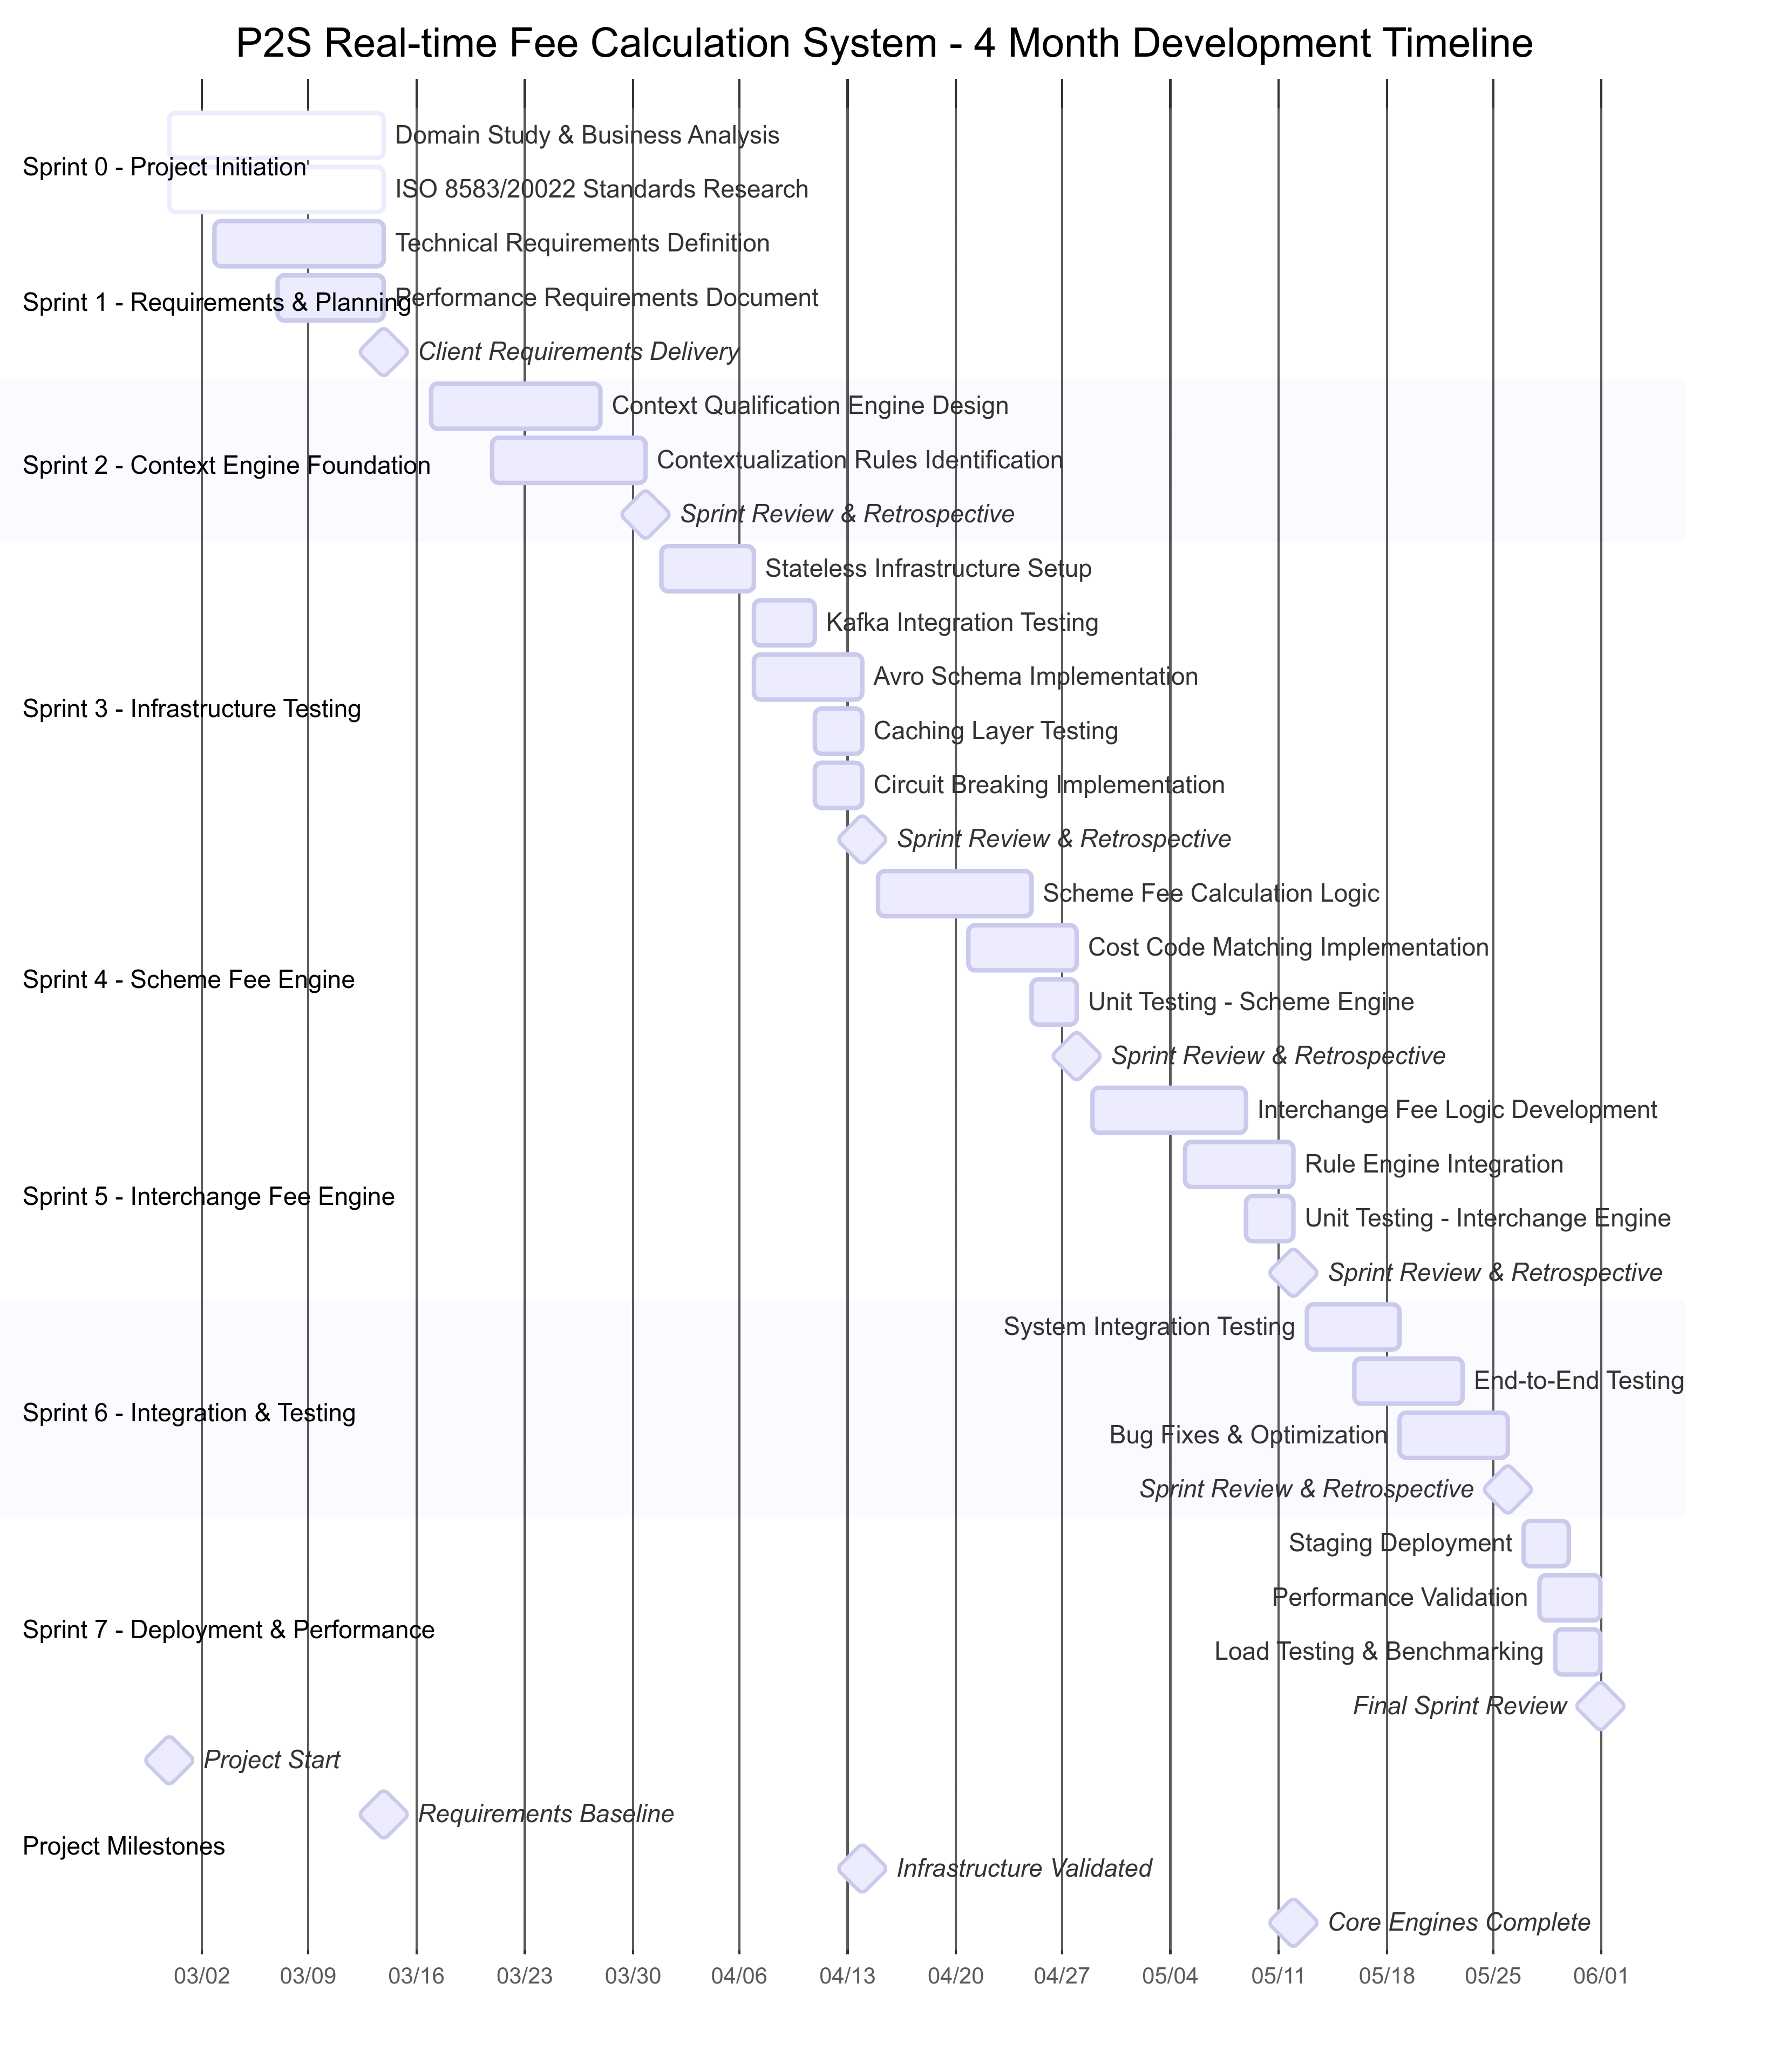
\includegraphics[width=\textwidth]{img/gantt.png}
    \caption{Project Timeline - Gantt Chart}
    \label{fig:gantt}
\end{figure}

\subsubsection{Sprint Structure}
\begin{itemize}
    \item \textbf{Sprint 0-1:} Project initiation and requirements definition
    \item \textbf{Sprint 2-3:} Context engine development and infrastructure setup
    \item \textbf{Sprint 4-5:} Fee calculation engine implementation
    \item \textbf{Sprint 6-7:} Integration testing and deployment
\end{itemize}

\section{System Architecture}

\subsection{P2S Platform Overview}

The P2S (Payment Processing System) platform is a distributed, event-driven architecture designed for high-volume financial transaction processing. The platform employs a microservices framework enabling modular development and deployment of system components.

\subsection{Compute Engines Architecture}

The compute engines represent the core processing components of the P2S platform, responsible for real-time fee calculation based on normalized payment scheme rules. The architecture emphasizes stateless processing, horizontal scalability, and fault tolerance.

\section{Technical Stack}

\subsection{Core Development Platform}

\textbf{Java:} Primary programming language providing platform independence, strong type system, and extensive ecosystem for enterprise application development.

\textbf{Spring Boot:} Application framework enabling rapid development of microservices with auto-configuration, embedded servers, and production-ready features.

\subsection{Data Management}

\textbf{PostgreSQL:} Primary relational database for transactional data storage, providing ACID compliance and complex query support.

\textbf{Redis:} In-memory caching solution for frequently accessed data, reducing database load and improving response times.

\subsection{Event Processing}

\textbf{Apache Kafka:} Distributed event streaming platform for real-time data pipeline management and inter-service communication.

\textbf{Apache Avro:} Data serialization framework ensuring efficient data exchange and schema evolution capabilities.

\textbf{Confluent Schema Registry:} Centralized schema management for Kafka topics, ensuring data consistency across microservices.

\subsection{Development Operations}

\textbf{GitLab:} Source code management and CI/CD pipeline automation for collaborative development and deployment.

\textbf{Docker:} Containerization platform ensuring consistent deployment environments and horizontal scaling capabilities.

\textbf{Apache Maven:} Build automation and dependency management for Java projects.

\section{Chapter Conclusion}

This chapter has established the comprehensive foundation for understanding the real-time fee calculation system development within the P2S financial platform. The analysis reveals that current payment processing systems face significant challenges in both structural representation of fee rules and computational efficiency in their application.

The identified problems - heterogeneous documentation formats and computational bottlenecks - directly impact operational efficiency and cost structures for financial institutions. The proposed solution addresses these challenges through an integrated framework combining systematic fee structure normalization with high-performance stateless computational engines.

Effyis Group provides an ideal environment for this project, with its specialized focus on payment systems and established P2S platform infrastructure. The company's flat organizational structure and agile development practices support the iterative approach necessary for complex financial system development.

The adoption of Scrum methodology ensures structured project management while maintaining flexibility for technical innovation. The comprehensive technical stack, centered on Java and Spring Boot with supporting technologies for data management and event processing, provides a robust foundation for implementing the proposed solution.

The next chapter will delve into the detailed analysis of existing fee calculation systems and the theoretical foundations underlying the proposed computational architecture, establishing the technical framework for the subsequent design and implementation phases.